\documentclass[tikz, dvisvgm, border=10pt]{standalone}
\usepackage{pgfplots}
\pgfplotsset{compat=1.18}

\begin{document}
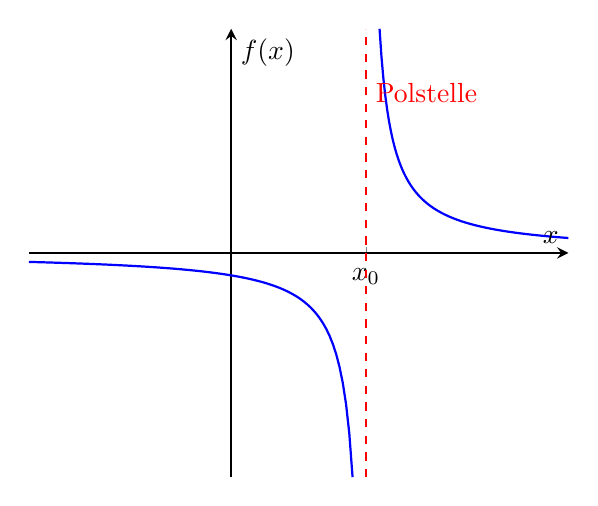
\begin{tikzpicture}
    \begin{axis}[
        axis lines = middle,
        xlabel = $x$,
        ylabel = {$f(x)$},
        ymin = -5, ymax = 5,
        xmin = -3, xmax = 5,
        xtick = {2},
        xticklabels = {$x_0$},
        ytick = \empty,
        grid = none,
        samples = 100,
        domain = -3:5,
        axis line style={thick},
    ]
        % The vertical asymptote (Polstelle)
        \draw [dashed, red, thick] (axis cs:2,-5) -- (axis cs:2,5);
        
        % The function: f(x) = 1/(x-2)
        \addplot [blue, thick, domain=-3:1.8] {1/(x-2)};
        \addplot [blue, thick, domain=2.2:5] {1/(x-2)};
        
        % Label for the asymptote
        \node [red, anchor=north west] at (axis cs:2, 4) {Polstelle};
    \end{axis}
\end{tikzpicture}
\end{document}